\documentclass[11pt,a4paper]{article}
\usepackage{graphicx}
\usepackage{xcolor}
\usepackage[utf8]{inputenc}
\usepackage{sectsty}
\usepackage[margin=25mm]{geometry}
\usepackage[utf8]{inputenc}
\usepackage{etoolbox}
\usepackage{parskip}
\usepackage{tikz}
\usepackage[english]{babel}
\usepackage{csquotes}
\usepackage{color, colortbl}
\usepackage{enumitem}
\usepackage{booktabs}
%\usepackage{cleveref}
\usepackage{subcaption}
\usepackage[margin=1cm]{caption}
\usepackage[colorlinks=true, breaklinks=false, urlcolor=blue, linkcolor=blue, allcolors=blue]{hyperref}
%\usepackage[backend=biber,style=numeric,sorting=none,autocite=plain]{biblatex}
%\addbibresource{references.bib}
\usepackage{harvard}
\usepackage{amsmath}
\usepackage{amssymb}
\usepackage{pgf}
\usepackage{graphicx}

\renewcommand{\baselinestretch}{1.5} 

\let\\=\relax % to ignore linebreak

\definecolor{Gray}{gray}{0.9}
\definecolor{LGray}{gray}{0.8}
\definecolor{HGray}{gray}{0.95}
\definecolor{pam_green}{HTML}{007373}

\sectionfont{\color{pam_green}}
\subsectionfont{\color{pam_green}}
\setlength{\parindent}{0pt}


% subtitle command
% /home/quants/git/quants-latex-rc/greenium_equity/greenium_paper.aux
\makeatletter
\providecommand{\subtitle}[1]{% add subtitle to \maketitle
	\apptocmd{\@title}{\par {\large #1}}{}{}
}
\makeatother

% keywords command
\providecommand{\keywords}[1]
{
	\small	
	\textbf{\textit{Keywords:}} #1
}

\title{\Large\textbf{\color{pam_green}A Forensic Analysis of ESG Risk Premia v1}}
\subtitle{\color{black}\textit{Pictet Asset Management - Multi Asset \& Quantitative Investment}}
\author{Sebastien Gorgoni, Remy Cottet and Olivier Monti}

\begin{document}

\begin{tikzpicture}[remember picture,overlay]
    \node[anchor=north west,yshift=80pt,xshift=-55pt]{\includegraphics[height=10mm]{figs/pam.png}};
\end{tikzpicture}

{\let\newpage\relax\maketitle}
\thispagestyle{empty}

\begin{abstract}
    \noindent
    In this paper we shed the light on the existence of an Environment, Social and Governance (ESG) equity risk premium. We first propose a methodology to build proprietary ESG ratings using data from independent providers.
    A standard risk-return framework is then applied to reveal any ESG risk premia from the perspective  of a beta aware investor considering the market only and a style aware investor accounting for the influence of sectors, country, market/fundamental factors and ESG factors.
    We analyze the existence of tilting opportunities on such ESG factors through an application to style factor long-short portfolio  
    This paper demonstrates the non-existence of ESG risk premia: after accounting for market beta, country, sector and style factor exposure, E/S/G factors did not historically generate persistent returns.
    Ignoring these exposures, a beta aware investor might mistakenly conclude the existence of ESG risk premia.
    The absence of ESG risk premia assumes the lack of influence of positive ESG tilts on performance, as empirically proven through style factor long-short portfolios.     
    This research  builds upon the work presented in \citeasnoun{kopp2021improve} by investigating the effect of ESG factors on long-only portfolio performance.
    The opinions expressed in this paper are solely those of the authors.
    There is an esg premia which disappear when controlling for known factors
    
\end{abstract}

\keywords{Risk Premia, ESG, Environment Social Governance, Sustainable Investing, Long Short Portfolios, Factor Investing, Factor Tilting.}

\clearpage

\tableofcontents

\clearpage

\section{Introduction}\label{sec:intro}

Given the expeditious growth of Environmental, Social and Governance (ESG) concerns in the asset management industry, asset managers might be open to understand the impact in their portfolios when taking into account this other-than financial metrics in the investment process. 
Multiple perspectives emerged while attempting to answer this question. On one hand, some advocate for the improved financial performance when considering companies with higher ESG-score, while others argue that performance remains unchanged regardless of ESG targets. Only a few have be arguing for the deterioration of results. 
However, many researches conducted on this issue fail to consider investments exposures on countries, sectors or \citeasnoun{fama1993common} risk factors exposures, leading to fallacious conclusions. 
Another challenge lies in the ESG score itself. As demonstrated by \citeasnoun{stackpole2021sustainable}, correlation among various providers has historically been as low as 0.61, contributing to inconsistent interpretations. 

Ultimatey, this research aims to uncover the pricing effects of  ESG scores on MSCI ACWI,  while acknowledging the aforementioned drawbacks. It seeks to address the following rhetorical question:

\medskip
\centerline{\textbf{Is there any ESG risk premia?}}
\medskip

It initially starts by establishing a robust framework for a proprietary methodology based on building blocks. 
These building blocks include blending the indicators obtained form independent data sources and in discounting the output based on the proportion of revenues obtained from controversial activities. 
The final score incorporate the ESG-related risks faced by the covered firm, as described in Section \ref{subsec:esg_data}.
The creation of proprietary ESG ratings is justified by the sense of obligation to address the growing concerns on ESG matters raised by both clients and regulatory authorities. 
The European Commission has actively responded to this by enforcing the Shareholder Rights Directive II of 2017 and the EU Sustainable Finance Disclosure Regulation (SFDR) of 2021. 
The former promotes effective and long-term shareholder participation in investment decision processes, while the latter establishes a transparent framework for ESG-related disclosure requirements.
The EU Green Taxonomy is expected to further increase the layer of sustainable-reporting. 
Consequently, ESG scores are  incorporated as independent inputs in the investment processes of managers of sustainable funds. 

To assess the existence of any ESG risk premia, a linear factor model is applied using two separate approaches to account the viewpoints of two distinct types of investors.
The first \textit{"naïve"} approach consider a direct pricing effect of the ESG scores on the investment universe's performance, net of market beta only. 
The second \textit{"multi-stage"} approach corresponds to an investor controlling for market beta as well as sector, country and risk/style factor exposures before uncovering any ESG risk premia. 
Results detailed in Section \ref{sec:res_factor} demonstrate the non-existence of ESG risk premia through the multi-stage approach, while the "naïve" beta-aware investor might mistakenly observe a positive risk premia as it fails to consider additional exposures that explain portfolio returns  
These findings are crucial for ESG investing, as they imply that a portfolio with a positive ESG tilt will deliver similar performance to a portfolio with no tilting. 

The aforementioned statement will be examined using long-short portfolios tilted to risk factors. Through these \textit{"pure style"} portfolios, a positive E/S/G bias will be enforced to assess any differences in performance. 
As shown in Section \ref{sec:res_lsptf}, increasing the E/S/G tilts on portfolios does not affect the performance of style factor portfolios.
This implies that portfolio managers can maintain their main style exposures and deliver similar risk-adjusted returns, while increasing the funds' weighted-average ESG scores by purchasing good/high ESG companies and selling poor/low ESG companies. 

As discussed in the literature review in Section \ref{sec:literature_review}, there is no clear consensus regarding whether ESG factors provide additional information in asset pricing models. 
The landscape seems unclear at first sight, and one reasonably questions the capacity of ESG factors to add independent and orthogonal pricing information not captured by the common style factors.
In fact, the literature addressing the global effects of ESG matters on financial performance can be approached by a binary perspective: either the consideration of the ESG dimension has a neutral effect on portfolio returns; or the ESG dimension exposes investors to a new and independent risk premium that must be taken into account. 
As this research attempts to identifies the pricing effect of ESG scores on forward returns through the aforementioned ESG risk premium paradigm, results presented in Section \ref{sec:res_factor} will confirm the conclusions of the first group.
Section \ref{sec:literature_review} provides a non-exhaustive overview of the literature on these two school of thoughts. 

\clearpage

\section{Literature Review}\label{sec:literature_review}

A plethora of research on the relationship between the inclusion of ESG metrics in investment processes and its effect on the financial performance has been made available to the public. 
In \citeasnoun{friede2015esg}, the authors aimed to evaluate the impact of ESG criteria on financial performance by examining over 2000 studies available on the topic.
The various studies found in academia can be categorized into two groups: the first one address the existence of a ESG risk premia, revealing the association between ESG ratings and financial performance, while the second focuses on the so-called "neutrality" of ESG factors, meaning their lack of impact on financial performance.
A review on both perspective 

\subsection{ESG Risk Premium}

The study presented in \citeasnoun{pollard2018establishing} uses the ESG ratings provided by MSCI to demonstrate that integrating them into a portfolio management strategy generates a premium independent to those of the Momentum, Volatility, Carry, Size, Value and Liquidity factors. 
Similarly, the work exposed in \citeasnoun{glossner2017esg} reveals the negative relationship between ESG risks and long-term returns. By using RepRisk's ratings, the author constructs low, medium and high ESG risk value-weighted portfolios while controlling for \citeasnoun{carhart1997persistence}'s four factor model, which includes the Beta, Size, Value and Momentum factors. 
As a result, the author finds that the portfolio with high ESG risks exhibits a negative alpha, even after controlling for industries or firm characteristics. Along with the ESG risk premium paradigm, the review presented in \citeasnoun{cornell2021esg} serves as a reminder that a significant number of studies indicates the significance of an ESG risk factor.
Controlling for size, industries and region, the research \citeasnoun{giese2019weighing} demonstrates that high ESG-rated companies exhibited higher profitability, paid higher dividends and had higher valuation levels between 2007 and 2017. 
In order to understand the relevance of ESG factors, \citeasnoun{nagy2016can} reveal that adopting either an ESG tilting or an ESG momentum strategy outperformed the benchmark. They further highlight that a significant part of this out-performance cannot be explained by style factors, suggesting the implicit and independent effects of ESG factors. 
Building upon this study, citeasnoun{maiti2021esg} uncover that a simple three factor model incorporating market, Size and ESG factors outperforms the Fama-French three factor model.
Additionally, \citeasnoun{lioui2018esg} assert that defensive equities, characterized by low volatility and/or low beta load, significantly align with the environment pillar. 
\citeasnoun{giese2016esg} integrate ESG factors into different smart Beta strategies and provide an explanation of how these factors should be used alongside common style factors in asset pricing models. 
Furthermore, by including ESG as an additional factor in the Fama-French three factor model augmented by momentum, and focusing on specific countries, the study conducted by \citeasnoun{sahut2015esg} finds that the variation of ESG scores is statistically significant in the UK, while it is not the case for the US and Switzerland. 
Taking another approach, \citeasnoun{kaiser2020esg} integrate environment, social and governance metrics into established investment processes and discover that value and growth investors can raise their sustainability ratings while improving their risk-adjusted performance, which it is not found to be the case for momentum investors. 

\subsection{ESG Neutrality}

Arguing against the influence of ESG ratings on portfolio performance, some highlight the fact that ESG factors become insignificant after controlling for multiple factors, as demonstrated in \citeasnoun{husse2021responsible}. 
The study conducted by \citeasnoun{bruno2022honey} supports the argument, revealing that while ESG strategies may appear attractive, they exhibit sector biased and are exposed to common equity risk premia. They also observe that as investors' appetite for ESG considerations increase, returns will be inflated. Furthermore, the performance of ESG momentum strategies has been flat since January 2008. 
In addition, the authors of \citeasnoun{bruder2019integration} establish a relationship between exposure of the Governance factor to the Quality factor in Europe. 
Moreover, studies affirming the absence of a relationship between ESG metrics in investment processes and the resulting financial performance can be found in \citeasnoun{friede2015esg}. 
In \citeasnoun{pastor2022dissecting}, it is noted that the recent high returns in green assets are not a consequence of high expected returns but rather stem from an increase in environmental concerns. They also estimate that green stocks carry a lower expected returns than brown stocks.
From a factor model perspective, the contribution of \citeasnoun{naffa2022factor} does not support the complementary of ESG factors to those included in the Fama-French five factor model (Beta, Size, Value, Profitability and Investment), supporting the argument of ESG neutrality. 
Additionally, \citeasnoun{amenc2021greeness} demonstrate that green stocks should yield lower returns than brown stocks as they provide risk-hedging benefits to the market, thus contradicting the assumption that any positive alpha is tied to green assets.
Regarding the intrinsic value of ESG ratings from third-party vendors, \citeasnoun{bams2022tilting} demonstrate that these ratings primarly reflect companies' sustainable objectives rather than actual performance. These objectives have proven not to be sustaible in the long-term as firms' reportins are often not standardized and lacks transparency.
Given the noiseness embedded in ESG ratings accross providers, \citeasnoun{berg2022esg} suggest methodology to correct for the noise. Without adjustments, the authors argue that the impact of ESG ratings on stock returns is underestimated by 60\%. 
Finally, the work detailed in \citeasnoun{dimson2020divergent} asserts that ESG ratings, when used in isolation, are unlikely to have a material contribution to portfolio returns.
Ultimately, arguing for the ESG neutrality would confirm the initial findings of \citeasnoun{kopp2021improve}, as investors can maintain the risk-adjusted performance of their portfolios unchanged while increasing their ESG tilts, thus highlighting the concept of "doing good whilst doing well" in investments. 

\clearpage

\section{Data}\label{sec:data}

This section defines the data and scope considered in this paper. It also introduce a methodology to establish a robust ESG score from external providers. 
Details on the systematic factors considered, both fundamental and market-based, are also presented.  

\subsection{Investment Universe}

To assess the existence of any ESG risk premia, the MSCI ACWI is being considered as the investable universe from 2007 to 2023. 
The monthly composition is taken into account, including information on its weight allocation, as well as each company details (i.e. sector, country, etc.) and its monthly returns. 

\subsection{Style Factors}\label{subsec:style_factor}

To maintain coherence throughout this paper, a distinction is made between \textit{Risk Premia} and\textit{Risk Factors}, as described by \citeasnoun{bender2013foundations}. 
Risk premia are risk factors that exhibit persistent premiums in the long-term due to their exposure to systematic risk: Fama-French factors are such examples.
On the other hand, "generic" risk factors, like liquidity and growth do no yield any persistent premiums in the long run. 
Throughout this paper, risk factors will often be denominated as \textit{Style Factors}.

To assess the existance of any ESG \textbf{risk premia}, the 12-month market beta is being considered, along with the prominent style factors from \textit{Axioma}. In particular, the considered ones are \textit{Value}, \textit{Size}, \textit{Momentum}, \textit{Volatility}, \textit{Quality}, \textit{Growth} and \textit{Liquidity} factors. 
The estimated factor returns shown in Figure \ref{fig:fmb_factor} demonstrate that some factors did earn premium consistently in the past. 
The market beta is determined empirically through an ordinary least square (OLS) regression with a one year rolling window given the MSCI ACWI daily returns as the dependent variable and the individual firms' daily returns as independent variables. 
To ensure consistency, the Value factor from Axioma, defined using the Book-to-Price ratio, is averaged with the Earning Yield factor, resulting in a custom factor that will still be referred to as the Value factor. 
The Quality factor is equivalent to the Profitability factor defined by Axioma. 

The factors are subsequently ranked in percentile in ascending order at each time step. 
They are then refined using a mapping from the inverse cumulative distribution function (ICDF) of the standard normal distribution, which is shown in Figure \ref{fig:icdf} of Appendix \ref{sec:icdf}. 
This process is analogous to assigning the corresponding z-score to each firm at each time step. 
% Since sector exposures are already considered as independent variables in the multi-step factor model described in Section \ref{sec:methodology}, the style factors are not sector-neutral. 
The z-scores are moreover winsorized such that they are all included in the $[-3,3]$ range. 

In summary, in addition of the market beta, this research consider seven fundamental and market-based risk factors well documented in the literature, characterized as z-scores.
Table \ref{tab:factors_summary} summarizes the set of factors:

\begin{center}
    \begin{tabular}{|l|p{5cm}|p{4cm}|p{3cm}|}
    \hline
    \rowcolor{LGray}
    \textbf{Factor} & \textbf{Description} & \textbf{Components} & \textbf{Category} \\
    \hline\hline
    Market Risk & Captures the sensitivity to overall market movements & 1-year rolling beta & Market-based \\
    \hline
    Momentum & Captures the trend or persistence in returns & 12-month cumulative returns & Market-based \\
    \hline
    Volatility & Measures the historical or expected price volatility & Volatility orthogonal to market sensitivity & Market-based \\
    \hline
    Size & Measures the relative size or market capitalization & Market capitalization (natural logarithm) & Market-based \\
    \hline
    Liquidity & Measures the ease of buying or selling securities & Trading volume, Amihud Ratio & Market-based \\
    \hline
    Value & Reflects the valuation based on fundamental factors (cheap vs. expensive stocks) & Price-to-book ratio; earnings yield & Fundamental-based \\
    \hline
    Quality & Reflects the financial strength and stability of companies & ROE, ROA, CF/Assets, CF/Income, Revenue/Assets, Gross margin & Fundamental-based \\
    \hline
    Growth & Reflects the expected or historical growth rates & Earnings growth, Revenue growth  & Fundamental-based \\
    \hline
\end{tabular}
    \captionof{table}{Market Risk \& Style Factors Summary}
    \label{tab:factors_summary}
\end{center}

Next section will decribe the methodology to develop the Environment, Social, Governance and overall ESG scores and factors, which are subjected to the same refining process.

\subsection{Proprietary ESG Scores \& Factors}\label{subsec:esg_data}

The methodology proposed to construct in-house proprietary ESG ratings defines the building blocks used for constructing Environment, Social and Governance ratings.
The overall ESG rating is evaluated by taking an equally-weighted average of the former individual pillars.
The proprietary ratings aim to establish a consensus view on concerns related to corporations along these three pillars. 
The guiding principles involve defining the scores as an expression of the ESG risk a company faces within each pillar. 
In this context, a low score indicates poor ESG credentials and, therefore, a high ESG risk.

As previously mentionned, ESG data has been found to be inconsistent across various prominent providers, with an average correlation of 0.61 \cite{stackpole2021sustainable}. 
Therefore, relying solely on one data provider for the research could lead to biased results. 
However, it is also important to note the limited availability of extensive historical ESG data. 
To address these issues, this paper proposes a blend of three major providers, stemming from the noise-correction methodology of ESG scores provided by \citeasnoun{berg2022esg}.

\begin{center}
    \begin{tabular}{||c c c||}
    \hline
    \rowcolor{LGray}
    \textbf{Provider} & \textbf{Variable} & \textbf{Inception date} \\ 
    \hline\hline
    MSCI & Environment Pillar Score & 2007-01-01 \\
    \hline
    MSCI & Social Pillar Score & 2007-01-01 \\
    \hline
    MSCI & Governance Pillar Score & 2007-01-01 \\
    \hline
    Inrate & Environment Grade & 2017-04-11 \\ 
    \hline
    Inrate & Society Grade & 2017-04-11 \\
    \hline
    Inrate & Governance Grade & 2017-04-11 \\
    \hline
    Sustainalytics & Environment Management Scores & 2020-07-09 \\
    \hline
    Sustainalytics & Social Management Scores & 2020-07-09  \\
    \hline
    Sustainalytics & Governance Management Scores & 2020-07-09  \\
    \hline
\end{tabular}

    \captionof{table}{ESG Data Providers}
    \label{tab:esg_data_provider}
\end{center}

The scoring methodology is detailed thereafter:
	
\begin{enumerate}
    \item \textit{Scaling}: The raw ESG scores for the historical MSCI ACWI universe, stemming from independent data providers, are mapped onto the $[0,10]$ range.
    \item \textit{Blending}: The scaled ratings are averaged to obtain a single rating for each of the Environment, Social and Governance pillars. As additional scores from a new provider are incorporated in the blending process, the average score may exhibit some fluctuations due to the relatively low correlation among providers. These anomalies are corrected. 
    \item \textit{Discounting}: This building block is twofold. It accounts both exclusions and involvements in selected controversial activities, as defined in the investment manager's responsible investment policy. Exclusions are addressed through a binary discounting, where the blended ratings are retained as they are if exclusions do not apply, or the rating is forced to zero otherwise. An exclusion is applied if a firm's revenue from a controversial activity exceeds certain predefined standards, if the firm is involved in a prohibited activity, if a firm has more than four controversies (as identified by Sustainalytics in this case) or if international standards are not met. Involvements in controversial activities that do not exceed the defined standards are considered in the second stage of the discounting process. Specifically, the revenues percentages derived from each controversial activity in which the firm is engaged are summed, and the sum is subtracted to 100\% in order to obtain the discount factor.
	\item \textit{Demeaning}: The difference of the score of each firm with the weighted-average of MSCI ACWI are added to the center of the $[0,10]$ range. After demeaning, the weighted score of the investment universe is hence always equal to 5. 
	\item \textit{Clipping}: If a demeaned rating is not contained in the $[0,10]$ range, its value is adjusted to the nearest bound. This adjustment is applied to the Environment, Social, Governance pillars.
    \item \textit{ESG Rating Generation}: The final stage involves creating the overall ESG scores based on the scores from the three pillars. The overall scores is determined at each point in time by taking the equal average of the Environment, Social and Governance scores.
\end{enumerate}

To assess the set of ESG factor exposures $F = \{E_F, S_F, G_F, ESG_F\}$ from the scores $\mathbb{S} = \{E, S, G, ESG\}$, the following steps are accomplished, where steps 2-4 are the same applied to the style factors in Section \ref{subsec:style_factor}.

\begin{enumerate}
    \item Standardization of style factors is considered good practice to obtain a common level of comparison among factors.
    The factors $F$ are determined by standardizing the scores $S$ at each point of time, as described in \ref{sec:stand_rf}.
    \item Factors $F$ are ranked in ascending order by percentile at each time $t$.
    \item The inverse cumulative distribution function (ICDF) of the standard normal distribution is applied.
    \item Lastly, the factors $F$, represented as z-scores, are windsorized to boung them within the range of $[-3,3]$.
\end{enumerate}

Finally, for the sake of conciseness throughout this paper, an \textit{ESG Risk Premia} will be conceptually defined as having a long position in good/high-ESG companies and a short position in poor/low-ESG companies. A positive/negative ESG risk premia is therefore defined as:
\begin{enumerate}
    \item \textbf{Positive ESG Risk Premia}: The portfolio is remunerated by having a \textit{long position in high-ESG} companies and a \textit{short position in low-ESG} companies.
    \item \textbf{Negative ESG Risk Premia}: The portfolio is remunerated by having a \textit{long position in low-ESG} companies and a \textit{short position in high-ESG} companies.
\end{enumerate}

\clearpage

\section{Methodology}\label{sec:methodology}

To evaluate the existence of any ESG risk premia in the equity space, this paper consider two approaches. The first approach involves a cross-sectional factor model, while the second considers long/short portfolios tilted with style factors.
These two methodologies can evaluate both the theoretical and practical materiality of ESG considerations in the investment industry. 

\subsection{Linear Cross-Sectional Factor Model}\label{subsec:fact_models}

As exposed in Section \ref{sec:intro}, the objective of this research is to determine whether ESG factors are priced in the returns of the investment universe and whether any risk premium can be demonstrated. Two approaches are considered through a cross-sectional regression:

\begin{enumerate}
    \item \textbf{Multi-Stage Approach:} This approach filters the information contained in the forward returns by sequentially removing the effects of the market beta, sectors, countries and style factors. It then evaluates the presence of any ESG greenium. 
    \item \textbf{Direct Approach:} This "naïve" version evaluate the pricing of ESG factors on the universe's forward returns directly after accounting for the market premium (beta), without considereing sectors, countries or style factors as described on Section \ref{subsec:style_factor}.
\end{enumerate}

Comparing these two approaches helps to determine whether any ESG risk premia truly exists in the investment universe or if other already well-known factors are crowding-out the expected ESG risk premia. 

\subsubsection{Factor Model}\label{subsec:fact_model}

The linear cross-sectional factor model used to evaluate the performance of a given set of factors consists of an Ordinary Least Squares (OLS) regression, which assumes the following form:

\begin{equation}
    R = F \phi + e
\end{equation}

\begin{equation}
    \begin{bmatrix} 
    R_{1}\\
    \vdots \\
    R_{n}
    \end{bmatrix}
    =
    \begin{bmatrix} 
    F_{1,1} & \dots  & F_{1,m}\\
    \vdots & \ddots & \vdots\\
    F_{n,1} & \dots  & F_{n,m} 
    \end{bmatrix}
    \begin{bmatrix} 
    \phi_{1}\\
    \vdots \\
    \phi_{m}
    \end{bmatrix}
    +
    \begin{bmatrix} 
    e_{1}\\
    \vdots \\
    e_{n}
    \end{bmatrix}
\end{equation}

At a given point in time, $F_{(N \times M)}$ is the exposure of factors $M={(0, ..., m)}$ for each asset $N={(0, ..., n)}$, $R_{(N \times 1)}$ is the matrix returns of the investment universe, $e_{(N \times 1)}$ is the residuals and $\phi_{(M \times 1)}$ is the returns of factor $M$. 
In this research, factor exposures are either characterized as z-scores of style/ESG factors or binary variables (i.e. country and sectors). 
 
The OLS estimation of the factor returns $\hat{\phi}$ is performed through a minimization of sum of squared residuals:
\begin{equation}
    \hat{\phi} = \mathrm{argmin} \left\| R - F \phi \right\|^2.
\end{equation}

Succinctly, the estimated returns are obtained in closed form as:

\begin{equation}
    \hat{\phi} = (F^\top F)^{-1} F^\top R
\end{equation}

\subsubsection{Multi-Stage Approach}\label{sec:multistage_model}

This approach comprises multiple stages of analysis, involving the use of of ordinary-least-quares (OLS) regressions, as described in Section \ref{subsec:fact_model}. 
These regressions are applied recursively on the residuals of the preceeding stage. 
This approach allows to reduce any multicollinearity issues among the independent variables. 
The objective is to capture the information in the forward returns that can be attributed to factors other than ESG, and then determine whether an orthogonal ESG pricing effect exists. 
The OLS regressions are performed cross-sectionally on a monthly basis. 
The analysis consists of five distinct stages.
	
\begin{itemize}[label=$\circ$]
    \item \textbf{Stage 1.} The market effect is removed from the monthly forward returns through 12-month rolling beta of the entire universe against the market. Additionally, these values are winsorized by two standard deviations in order to reduce the impact of outliers on the analyses. The residuals of this stage are used as an input of stage 2.
    \begin{equation}
        R = F_{\text{Market}} \phi_{\text{Market}} + e_{1}
    \end{equation}
    \item \textbf{Stage 2.} The sector bias is removed. The OLS considers dummy variables in order to account for each of the GICS level 1 sectors, where $F_{text{Sector}}\in \{0, 1\}$ is a binary matrix. The residuals of this stage are used as an input of stage 3.
    \begin{equation}
        e_{1} = F_{\text{Sector}} \phi_{\text{Sector}} + e_{2}
    \end{equation}
    \item \textbf{Stage 3.} The third stage removes the pricing effect of all countries in the universe, where $F_{text{Country}}\in \{0, 1\}$ is a binary matrix. This OLS also considers only dummy independent variables in the estimation.
    \begin{equation}
        e_{2} = F_{\text{Country}} \phi_{\text{Country}} + e_{3}
    \end{equation}
    \item \textbf{Stage 4.} This stage removes the effects of the style factors described in Section \ref{subsec:style_factor} on the residuals of the third stage. The style factors are characterized as z-scores.
    Concerns on any multicolinearity issues are low given the overall low correlations among the style factor exposures,  as shown in Figure \ref{fig:fmb_factor_z_corr}. The residuals are sent as input to the final stage.
    \begin{equation}
        e_{3} = F_{\text{Style}} \phi_{\text{Style}} + e_{4}
    \end{equation}   
    \item \textbf{Stage 5.} This stage considers the effect of the Environment, Social and Governance factors or overall ESG factor on the residuals of the fourth stage. 
    The three pillars are considered together as independent variables of the same cross sectional OLS regression due to their low correlation, as shown in Figure \ref{fig:fmb_factor_z_corr}, reducing any concerns of multicolinearity. 
    Another distinct regression is performed, considering solely the overall ESG factor to avoid any multicollinearity issues.
    \begin{equation}
        e_{4} = F_{\text{\{E/S/G; ESG\}}} \phi_{\text{\{E/S/G; ESG\}}} + e_{5}
    \end{equation}  
\end{itemize}

\begin{figure}[h!] 
    \centering
    \includegraphics[width=1\textwidth]{figs/fmb/factor_z_corr.png} 
    \caption{Factor Exposure (Z-Scores) Correlation Matrix}
    \label{fig:fmb_factor_z_corr}
\end{figure}

A common issue when including binary independent variables in an OLS regression, such as stages 2 and 3, is that one of the features will be arbitrary absorbed into the regression's constant, in addition to potential multicollinearity concerns.
To tackle these issues, a straightforward approach is to enforce the sum of factor returns to be equal to zero, as described by \citeasnoun{menchero2010characteristics} and \citeasnoun{axioma2017model}.

\begin{equation}
    \sum_{i=1}^{N}{w_{i}\phi = 0}
\end{equation}

Usually, market capitalization is considered to determine the regression weights $w_{i}$.

\subsubsection{Direct Approach}

The second approach is a segmentation of the first one. It applies the first stage directly followed by the fifth stage. 
This approach represents the simplest and most hazardous method to assess the existence of an ESG risk premium.

\subsection{Long-Short Portfolio Model}\label{sec:methodo_lsptf}

While a linear factor model provides a robust methodology for assessing the presence of a risk premium, its implications remain conceptual and challenging to integrate into realistic scenarios because the implied portfolios are not tradable. 
Therefore, this section presents a more practical approach by constructing long/short portfolios that are tilted with style factors, as described in Section \ref{subsec:style_factor}, while varying the level of appetite for E-S-G scores. 
The portfolios will be neutral with respect to beta, sectors, countries, and style factor exposure, except for the factor to which the portfolio is tilted. 
In contrast to the approach described in \citeasnoun{kopp2021improve}, this method will demonstrate that the performance of portfolios will neither improve nor worsen when there is a positive bias towards E/S/G by favoring good ESG companies and penalizing poor ones, while maintaining the same style exposure target.

To build such models, optimized mean-variance portfolios are estimated as follow: 

\begin{equation}
    \begin{aligned}
    \max_{w} \quad & \lambda_{F_{T}} w'F_{T} + \lambda_{\mathbb{S}} w'\mathbb{S} - \lambda_{\Sigma}w'\Sigma w\\
    \textrm{s.t.} \quad & \sum_{i=1}^{N}{w_{i}\beta_{i}} = 0 \\
    & \sum_{i=1}^{N}{w_{i}\beta_{i}M_{Sector}} = 0 \\
    & \sum_{i=1}^{N}{w_{i}\beta_{i}M_{Country}} = 0 \\
    & \sum_{i=1}^{N}{w_{i}F} = 0,  F_{T} \notin F \\
    & \sum_{i=1}^{N}{w_{i}} = 0 \\
    & \sum_{i=1}^{N}{\left|w_{i}\right|} \leq 2 \\
    & \sum_{i=1}^{N}{w_{i}\mathbb{S}_{i}} \geq 0 \\
    & -0.05 \leq w_i\leq 0.05 \\
    \end{aligned}
\end{equation}

This approach has been designed to maximize the weighted average exposure of the target style factor exposure $F_{T}$ while simultaneously minimize the portfolio's volatility, 
captured through the covariance matrix $\Sigma$. The covariance matrix has been shrunked, to reduce the impany of potential noisy data.
The shrinkage approach follows principal component analysis in which it selects the factors which explain 90 percent of the variance. 
The set of considered style factors are defined in Section \ref{subsec:style_factor}.
ESG considerations can be evaluated using the weighted average score $\mathbb{S} = \left(E, S, G \right)$, while the level of preference for ESG can be determined by $\lambda_{\mathbb{S}}$. 
Therefore this approach allows for a trade-off between factor exposure $\lambda_{F_{T}}$, E/S/G bias $\lambda_{\mathbb{S}}$ and risk $\lambda_{TE}$. 
For simplicity, $\lambda_{\mu}$, $\lambda_{\mathbb{S}}$ and $\lambda_{TE}$ are arbitrarily fixed, were $\lambda_{\mathbb{S}} < \lambda_{F_{T}} < \lambda_{TE}$.
$M_{Sector}$ and  $M_{Country}$ are binary matrices determining whether a company operates within a given sector/country. 
Additionally, due to the convex nature of this optimization problem, the state-of-the-art model developed by \citeasnoun{ali2015disciplined} has been used to construct portfolios. 
Finally, rebalancing is done monthly while assuming a trading fee of 5 basis points (bps). 

\clearpage

\section{Results}

\subsection{ESG Risk Premia Estimation}\label{sec:res_factor}

This section presents the results obtained from the cross-sectional factor model described in Section \ref{subsec:fact_model}. The findings serve as strong conceptual evidence for the non-existence of ESG risk premia, which will be further demonstrated in practical applications discussed in Section \ref{sec:res_lsptf}. 

\subsubsection{Linear Factor Model Results}

In the first stage of both the direct and multi-stage approaches, the linear cross-sectional factor model is employed. This model considers the forward returns of the assets in the universe as the dependent variable and their beta as the independent variable.
Figure \ref{fig:fmb_beta} illustrates the estimated cumulative returns of the MSCI ACWI market beta.

\begin{figure}[h!] 
    \centering
    \includegraphics[width=0.6\textwidth]{figs/fmb/fmb_beta.png}
    \caption{Cumulative Returns of Sectors (Multi-Stage Approach)}
    \label{fig:fmb_beta}
\end{figure}

Through the multi-stage approach, the second stage aims to eliminate the impact of sectors on asset performance. 
This is achieved by using the residuals from the first stage as the dependent variable and assigning a dummy variable to each sector, except for one. 
This allows for cross-sectional OLS regressions to capture the respective influences of each sector. 
Consequently, this stage determines the sensitivity of market dynamics to sector performance at each time step and removes their influence before passing the residuals as input to the third stage.
Figure \ref{fig:fmb_sector} displays the cumulative performance of sector returns. 
As observed, Information Technology and Health Care have experienced the most significant rally since 2007, while Energy and Real Estate have faced substantial drawdowns.

\clearpage

\begin{figure}[h!] 
    \centering
    \includegraphics[width=0.7\textwidth]{figs/fmb/fmb_sector.png}
    \caption{Cumulative Returns of Style Factors (Multi-Stage Approach)}
    \label{fig:fmb_sector}
\end{figure}

The third stage replicates the second stage but replaces the sector dummies with the countries of the assets in the investment universe.
Figure \ref{fig:fmb_country} illustrates the evolution of country returns, which are determined from regressions that use the residuals from the second stage as the dependent variable and the country dummies as independent variables.

\begin{figure}[h!]
    \centering
    \begin{subfigure}{.5\textwidth}
        \centering
        \includegraphics[width=1\linewidth]{figs/fmb/fmb_country_ameeur.png}
        \caption{Americas \& Europe}
        \label{fig:fmb_country_ameeur}
    \end{subfigure}%
    \begin{subfigure}{.5\textwidth}
      \centering
      \includegraphics[width=1\linewidth]{figs/fmb/fmb_country_midpac.png}
      \caption{Asia, Middle-East \& Pacific}
      \label{fig:fmb_country_midpac}
    \end{subfigure}
    \caption{Cumulative Returns of Country Exposures}
    \label{fig:fmb_country}
\end{figure}

Before the final stage of the multi-stage analysis, the impact of style returns on the financial performance of assets is removed, taking into account market beta (stage 1), sectors (stage 2), and countries (stage 3).
Figure \ref{fig:fmb_factor} showcases the cumulative values of estimated factor returns within MSCI ACWI. 
The results demonstrate that certain factors, such as momentum, volatility, quality, and value, have consistently provided positive returns since 2008. However, other factors, including growth, liquidity, and size, have not yielded consistent premia.

\begin{figure}[h!] 
    \centering
    \includegraphics[width=0.7\textwidth]{figs/fmb/fmb_stylefactor.png}
    \caption{Cumulative Returns of Style Factors (Multi-Stage Approach)}
    \label{fig:fmb_factor}
\end{figure}

By removing the aforementioned effects from the returns of the investment universe, it allows to directly compare the multi-stage approach with the direct approach. 
The direct approach, often referred as the "naïve" version, only accounts for the market beta exposure.
Figures \ref{fig:fmb_esg} and \ref{fig:fmb_esg_DA} illustrate the estimated cumulative returns of the ESG factor for both approaches. 
These figures suggest that the initial conclusions drawn from the direct approach, which indicate a positive ESG risk premia, is annuled when sector, country, and factor style exposures are included in the analysis.
In fact, when these factors are taken into consideration, the cumulative returns of these pillars have remained relatively stagnant since 2007, \footnote{Same scales have been applied from Figures \ref{fig:fmb_factor} to \ref{fig:fmb_e_s_g} for comparability purposes.} indicating the absence of ESG risk premia. 

\begin{figure}[h!]
    \centering
    \begin{subfigure}{.5\textwidth}
        \centering
        \includegraphics[width=1\linewidth]{figs/fmb/fmb_esg_DA.png}
        \caption{Direct Approach}
        \label{fig:fmb_esg_DA}
    \end{subfigure}%
    \begin{subfigure}{.5\textwidth}
      \centering
      \includegraphics[width=1\linewidth]{figs/fmb/fmb_esg.png}
      \caption{Multi-Stage Approach}
      \label{fig:fmb_esg}
    \end{subfigure}
    \caption{Cumulative Returns of ESG Factors}
\end{figure}

Most of the positive cumulative returns observed in the ESG factor using the naïve approach can be attributed to the Governance factor, with some contribution from the Environment factor, as depicted in Figure \ref{fig:fmb_e_s_g_DA}
Through the multi-stage approach, the environment and governance factors are being crowded out by a blend of exposures (i.e., country, sector, style), similar to the overall ESG factor. 
Interestingly, the returns of the S factor remain relatively stable for both approaches, indicating that, overall, it is not significantly influenced by the other factors examined in this study. 
Nevertheless, it is worth noting that the direct approach shows some positive returns for this factor since 2019, which warrants further analysis. 
Section \ref{subsec:fact_dec} will delve into this matter.

\begin{figure}[h!]
    \centering
    \begin{subfigure}{.5\textwidth}
        \centering
        \includegraphics[width=1\linewidth]{figs/fmb/fmb_e_s_g_DA.png}
        \caption{Direct Approach}
        \label{fig:fmb_e_s_g_DA}
    \end{subfigure}%
    \begin{subfigure}{.5\textwidth}
      \centering
      \includegraphics[width=1\linewidth]{figs/fmb/fmb_e_s_g.png}
      \caption{Multi-Stage Approach}
      \label{fig:fmb_e_s_g}
    \end{subfigure}
    \caption{Cumulative Returns of E/S/G Factors}
\end{figure}

\clearpage

\subsubsection{Long-Term Factor Decomposition}\label{subsec:fact_dec}

This section aims to determine which factor(s) are responsible for crowding out the positive cumulative returns of the E/S/G factors in the direct approach.
Figure \ref{fig:fmb_decomp} depict such decomposition analysis, net of \textit{Beta} for all charts.
Another method to decompose the E/S/G factors is to determine its performance after sequentially accounting for all sector, country and style exposures, following the multi-stage approach defined in section \ref{sec:multistage_model}.
Figure \ref{fig:fmb_factor_ret_corr} illustrates the correlation matrix of all estimated factors' returns, except countries.
The correlation matrix between ESG factors and countries has been included in the appendix \ref{appendix:corr_country_esg} due to visualization purposes. 
The naïve approach's risk premium for the Governance factor appears to be primarily influenced by country exposures and style factors. 
This finding is not surprising, considering that governance practices can be influenced by cultural differences across countries.
Sector exposure and style factors prove to be the most influential variables in explaining the naïve approach's risk premium for the Environment factor, providing insights into the relationship between carbon-intensive industries and environmental factors. 
Notably, Figure \ref{fig:fmb_factor_ret_corr} demonstrates significant negative correlations between the environmental factor and the energy as well as materials sectors. 
While the social factor remains relatively stable in both the direct and multi-stage approaches, it appears to be marginally influenced, either positively or negatively, by other explanatory factors. 
However, the overall effects remain relatively flat.
Lastly, the aggregated ESG factor is logically affected by all country, sector and style factors exposures.
Noteworthy findings include significant negative correlations with energy and materials companies and positive correlations with volatility and quality styles. 

\begin{figure}[h!]
    \centering
    \begin{subfigure}{.33\textwidth}
        \centering
        \includegraphics[width=1\linewidth]{figs/fmb/fmb_D_S.png}
        \caption{Net of Sector Factors}
        \label{fig:fmb_D_S}
    \end{subfigure}%
    \begin{subfigure}{.33\textwidth}
      \centering
      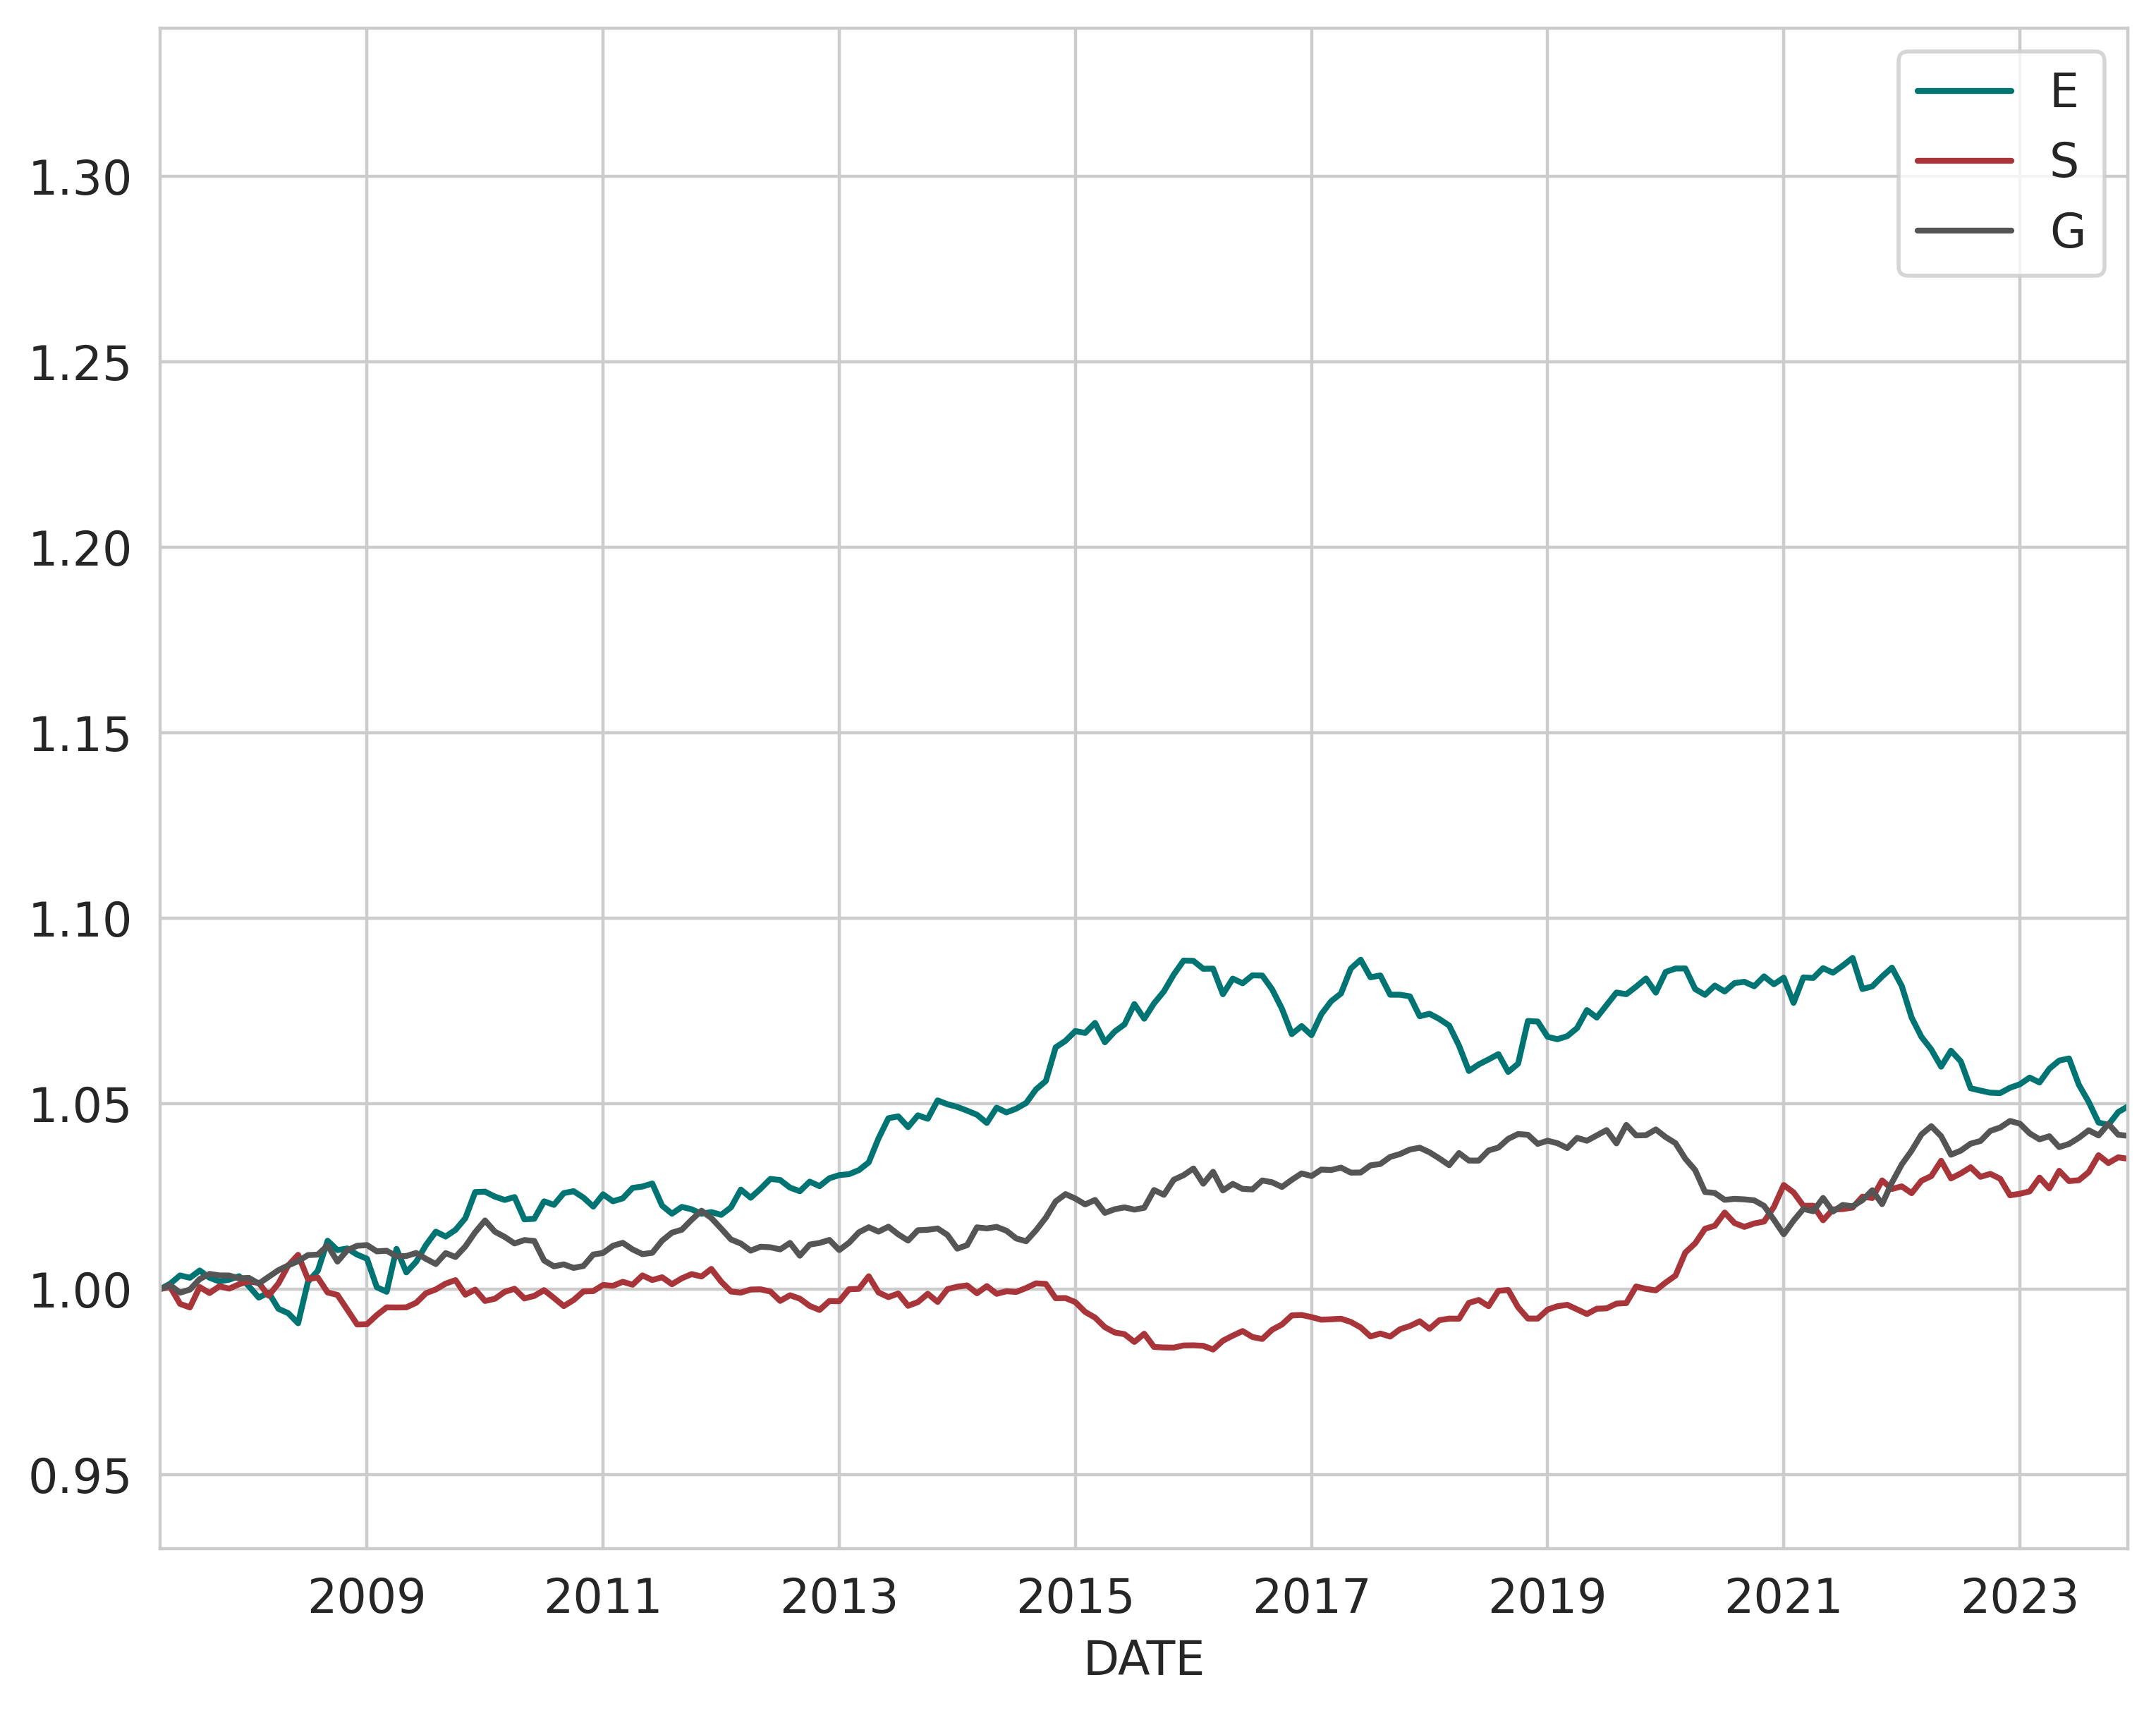
\includegraphics[width=1\linewidth]{figs/fmb/fmb_D_C.png}
      \caption{Net of Country Factors}
      \label{fig:fmb_D_C}
    \end{subfigure}%
    \begin{subfigure}{.33\textwidth}
        \centering
        \includegraphics[width=1\linewidth]{figs/fmb/fmb_D_F.png}
        \caption{Net of Style Factors}
        \label{fig:fmb_D_F}
      \end{subfigure}
    \caption{Cumulative Returns of E/S/G Factors}
    \label{fig:fmb_decomp}
\end{figure}

\clearpage

\begin{figure}[h!]
    \centering
    \begin{subfigure}{\textwidth}
        \centering
        \includegraphics[width=0.8\linewidth]{figs/fmb/fmb_seq_e.png}
        \caption{Environmental Factor}
    \end{subfigure}
    \begin{subfigure}{\textwidth}
      \centering
      \includegraphics[width=0.8\linewidth]{figs/fmb/fmb_seq_s.png}
      \caption{Social Factor}
    \end{subfigure}
    \begin{subfigure}{\textwidth}
        \centering
        \includegraphics[width=0.8\linewidth]{figs/fmb/fmb_seq_g.png}
        \caption{Governance Factor}
      \end{subfigure}
    \caption{Cumulative Returns of E/S/G Factors: Sequential Decomposition}
\end{figure}

\clearpage

\begin{figure}[h!] 
    \centering
    \includegraphics[width=1.5\textwidth,angle=90,origin=c]{figs/fmb/factor_ret_corr.png} 
    \caption{Factor Returns Correlation Matrix}
    \label{fig:fmb_factor_ret_corr}
\end{figure}

\clearpage

\subsubsection{Summary}

To summarize the key findings discussed in the preceding two sections, which were derived from the two approaches outlined in Section \ref{subsec:fact_models}, the main distinction between the two approaches lies in the omission of considering the impacts of sectors, countries, and style factors on the financial performance of assets.
Table \ref{tab:fmb_esgpremia_summary} provides an overview of the main findings associated with the two approaches.

\begin{center}
    \begin{tabular}{||c c c c||} 
    \hline
    \rowcolor{LGray}
    \textbf{Factor} & \textbf{Cumulative Returns} & \textbf{Risk premium} & \textbf{Crowding-Out Factors}\\
    \hline\hline
    \rowcolor{Gray}
    \multicolumn{4}{||c||}{\textit{Multiple Stage Approach}} \\
    \hline\hline
    Environment & Flat & Neutral & Sectors \& Styles \\ 
    \hline
    Social & Flat & Neutral & Countries, Sectors \& Styles \\
    \hline
    Governance & Flat & Neutral & Countries \& Styles \\
    \hline
    ESG & Flat & Neutral  & Countries, Sectors \& Styles \\ 
    \hline\hline
    \rowcolor{Gray}
    \multicolumn{4}{||c||}{\textit{Direct Approach}} \\
    \hline\hline
    Environment & Increase & Positive & - \\ 
    \hline
    Social & Slight Increase (since 2019) & Neutral & - \\
    \hline
    Governance & Increase & Positive & - \\
    \hline
    ESG & Increase & Positive & - \\ 
    \hline
\end{tabular}
    \captionof{table}{Summary of ESG Risk Premia Estimation}
    \label{tab:fmb_esgpremia_summary}   
\end{center}

\subsubsection*{\textit{Environmental}}

A naïve investor would quickly conclude the existence of an environmental risk premium based on the persistent positive cumulative returns shown in Figure \ref{fig:fmb_e_s_g_DA}. 
The majority of these positive returns were generated between 2013 and 2016, after which they remained relatively flat.
However, this conclusion is flawed as it fails to consider significant exposures such as countries, sectors, and style factors. 
When accounting for these factors, as shown in Figure \ref{fig:fmb_e_s_g}, the cumulative returns flatten out, suggesting the absence of an environmental risk premium.
The outperformance observed in the direct approach is largely offset by exposures to sectors and style factors.
Specifically, the "naïve" E risk factor exhibits a strong positive correlation with specific defensive sectors (i.e., consumer staples and healthcare) and cyclical sectors (i.e., communication services, consumer discretionary and industrials), while displaying a negative correlation with carbon-intensive companies (e.g., energy and materials). 
Additionally, the E risk factor demonstrates a positive correlation with the low volatility and quality factors, coinciding with its exposure to these aforementioned defensive sectors. 

\subsubsection*{\textit{Social}}

The social factor stands out as the only factor that has not generated persistent positive cumulative returns for both approaches since 2007. 
However, the direct approach shows a slight increase in cumulative returns since 2019, which can be attributed to its positive correlation with the energy sector.
Furthermore, Figure \ref{fig:fmb_factor_ret_corr} illustrates a strong positive correlation between the social factor and consumer staples.
Figures \ref{fig:fmb_decomp} demonstrate that when accounting for various exposures, the impact on estimated returns can be either positive, negative, or neutral, resulting in a net neutral effect.

\subsubsection*{\textit{Governance}}

Similar to the environmental factor, the direct approach may incorrectly conclude the existence of a positive governance risk premium. 
Figure \ref{fig:fmb_e_s_g_DA} shows a significant positive outperformance, particularly since 2021.
However, most of these outperformances can be attributed to country exposures, as demonstrated in Figure \ref{fig:fmb_D_C}, which are influenced different corporate cultures across the globe.
Furthermore, the low volatility factor can also significantly account for these outperformances. 
A company with strong governance practices may, for instance, prioritize maintaining a stable stock price and limiting fluctuations by avoiding excessive investments.

\subsubsection*{\textit{Overall ESG}}

As depicted in Figure \ref{fig:fmb_esg}, the direct approach also estimate a positive overall ESG risk premia. 
This positive outperformance can naturally be attributed to a combination of the same exposures within each of the E/S/G pillars.
Similar to the E factor, ESG performance shows a positive correlation with defensive sectors such as consumer staples and healthcare, while displaying a negative correlation with carbon-intensive sectors like energy and materials.
Additionally, similar positive correlation is displayed for cyclical sectors. 
Furthermore, Figure \ref{fig:fmb_factor_ret_corr} demonstrates a positive correlation with the low volatility and quality factors. 
Finally, it is important to note that the ESG factor may also be influcenced by structural differences between countries, crowding-out the naïve ESG risk premium.

\clearpage

\subsection{Long-Short ESG Portfolios}\label{sec:res_lsptf}

The findings presented in Section \ref{sec:res_factor} hold significant ramifications for ESG investing. 
Based on the conclusion that the ESG risk premium has historically been nonexistent, \textit{investors should not anticipate being rewarded or penalized solely by tilting their portfolios based on ESG scores}.
This implies that investors can increase their positive ESG exposure without sacrificing risk-adjusted performance or deviating from their desired style, country, and sector allocations.
While these findings are meaningful, they are still conceptual in nature since the portfolios derived from the estimated returns are not tradable.
This section provides a comprehensive analysis on the implications of the results outlined in Section \ref{sec:res_factor} by constructing long-short style factors portfolio with ESG bias.
Through a long-short approach, the equity portfolio will reward high-ESG companies while penalizing low-ESG companies, thereby encompassing the entire spectrum of ESG investments. This is in contrast to the approach taken by \citeasnoun{kopp2021improve}, who only consider long-only portfolios without style exposure control.

For the sake of conciseness, only two style portfolios will be presented based on performamce and the underlying data: low-volatility factor (market-based) and quality factor (fundamental-based).   
Results from the other style portfolios are included in Appendix \ref{appendix:ls_ptf_res}: conclusions remain however valid for all portfolios. 

\subsubsection{Low Volatility Portfolio (Market-Based)}

A long-short volatility portfolio aims to hold long positions into stocks with low-volatility and short-positions in stocks with high-volatility. 
As shown in Figure \ref{fig:fmb_factor}, this style factor has consistently delivered a positive risk premium over time, suggesting that exposing a portfolio to such risk factor could improve its performance.
Without imposing any E/S/G bias, the cumulative performance of this \textit{pure style} strategy, considering the set of constraints explained in Section \ref{sec:methodo_lsptf}, is displayed in Figure \ref{fig:vol_cumret}.
This portfolio has historically delivered satisfactory performance, highlighting the attractiveness of being exposed to low-volatility stocks.
By introducing an E/S/G bias, Figure \ref{fig:vol_cumret} demonstrates an overall increase of cumulative returns from 2007 to 2023, suggesting an improvement in raw returns by incorporating positive tilts towards the E/S/G scores.
However, when examining in excess of the \textit{pure style} portfolios' returns in Figure \ref{fig:vol_cumexret}, it becomes evident that most of the outperformance occurred until 2015. Since then, portfolios with an E/S/G bias have underperformed the \textit{pure style} portfolio.
The lack of consistent performance over time for a low-volatility portfolio with increasing positive E/S/G tilts does not allow for a definitive conclusion regarding persistent outperformance or underperformance.
Additionally, these portfolios have generated similar risk-adjusted performance compared to the \textit{pure style} portfolio.    

\begin{figure}[h!]
    \centering
    \begin{subfigure}{.5\textwidth}
        \centering
        \includegraphics[width=1\linewidth]{figs/ls/vol_cumret.png}
        \caption{Cumulative Returns}
        \label{fig:vol_cumret}
    \end{subfigure}%
    \begin{subfigure}{.5\textwidth}
      \centering
      \includegraphics[width=1\linewidth]{figs/ls/vol_cumexret.png}
      \caption{Cumulative Excess Returns}
      \label{fig:vol_cumexret}
    \end{subfigure}
    \caption{L/S Volatility Portfolio: Performance}
\end{figure}

\begin{center}
    \begin{tabular}{lcccc}
\toprule
 & E Bias & S Bias & G Bias & Pure Style \\
\midrule
Ann. Rtn (\%) & 4.5 & 4.5 & 4.9 & 4.1 \\
Cum. Rtn (\%) & 113.8 & 116.1 & 128.6 & 100.2 \\
Avg. Rtn (\%) & 5.1 & 5.2 & 5.5 & 4.8 \\
Vol. (\%) & 12.2 & 12.2 & 12.2 & 12.3 \\
Max DD (\%) & -33.5 & -38.5 & -37.6 & -33.7 \\
Sharpe Ratio & 0.4 & 0.4 & 0.5 & 0.4 \\
Sortino Ratio & 0.6 & 0.6 & 0.7 & 0.6 \\
Calmar Ratio & 0.1 & 0.1 & 0.1 & 0.1 \\
Skew & 0.0 & -0.0 & -0.1 & 0.0 \\
Kurtosis & 1.2 & 1.4 & 1.2 & 1.6 \\
Turnover & 16.6 & 16.5 & 16.6 & 16.4 \\
\bottomrule
\end{tabular}

    \captionof{table}{Volatility L/S Portfolio: Statistics}
    \label{tab:vol_stats}
\end{center}

Despite these results, Figure \ref{fig:vol_esg_wa} demonstrates that increasing the portfolio's E/S/G score does not have a significant impact on its performance. 
The portfolios with bias have been able to generate similar risk-adjusted returns while maintaining a consistent positive E/S/G tilt compared to the \textit{pure style} portfolio.

\begin{figure}[h!]
    \centering
    \begin{subfigure}{.33\textwidth}
        \centering
        \includegraphics[width=1\linewidth]{figs/ls/vol_e_wa.png}
        \caption{Environment}
        \label{fig:vol_e_wa}
    \end{subfigure}%
    \begin{subfigure}{.33\textwidth}
      \centering
      \includegraphics[width=1\linewidth]{figs/ls/vol_s_wa.png}
      \caption{Social}
      \label{fig:vol_s_wa}
    \end{subfigure}%
    \begin{subfigure}{.33\textwidth}
        \centering
        \includegraphics[width=1\linewidth]{figs/ls/vol_g_wa.png}
        \caption{Governance}
        \label{fig:vol_g_wa}
      \end{subfigure}
    \caption{L/S Volatility Portfolio: Weighted-Average E/S/G Scores}
    \label{fig:vol_esg_wa}
\end{figure}

The results obtained from the low-volatility long/short portfolios remain valid for the other market-based portfolios considered in this research (i.e. momentum, size and liquidity). 

\subsubsection{Quality Portfolio (Fundamental-Based)}

Within a long-short quality portfolio, stable companies with strong financials are bought while companies with weak financials are sold. The stock selection is based on either an unique or a blended set of fundamental metrics such as ROA, ROE, Gross Margin and others.
Similarl to the volatility factor, the quality factor has consistently delivered positive returns over time, indicating that exposure to quality companies should provide positive risk premiums to investors.
As shown in figure \ref{fig:qua_cumret}, incorportating an environmental or social bias increases the portfolio's net cumulative return, except for ther governance bias, where performance is similar to the \textit{pure style} portfolio. 
However, most of this outperformance for can be attributed by positive excess returns until 2015 compared to the \textit{pure style} portfolio. 
Since then, excess returns have been on average negligible, and the portfolio with a governance bias have been underperforming since 2013. 
These results also suggest that an increase in E/G/S tilts does not have any significant impact on average in the quality portfolio's performance. 
However, the weighted-average E/S/G scores of these biased portfolios remain consistently higher compared to the \textit{pure style} portfolio.

\begin{figure}[h!]
    \centering
    \begin{subfigure}{.5\textwidth}
        \centering
        \includegraphics[width=1\linewidth]{figs/ls/qua_cumret.png}
        \caption{Cumulative Returns}
        \label{fig:qua_cumret}
    \end{subfigure}%
    \begin{subfigure}{.5\textwidth}
      \centering
      \includegraphics[width=1\linewidth]{figs/ls/qua_cumexret.png}
      \caption{Cumulative Excess Returns}
      \label{fig:qua_cumexret}
    \end{subfigure}
    \caption{L/S Quality Portfolio: Performance}
\end{figure}

\begin{figure}[h!]
    \centering
    \begin{subfigure}{.33\textwidth}
        \centering
        \includegraphics[width=1\linewidth]{figs/ls/qua_e_wa.png}
        \caption{Environment}
        \label{fig:qua_e_wa}
    \end{subfigure}%
    \begin{subfigure}{.33\textwidth}
      \centering
      \includegraphics[width=1\linewidth]{figs/ls/qua_s_wa.png}
      \caption{Social}
      \label{fig:qua_s_wa}
    \end{subfigure}%
    \begin{subfigure}{.33\textwidth}
        \centering
        \includegraphics[width=1\linewidth]{figs/ls/qua_g_wa.png}
        \caption{Governance}
        \label{fig:qua_g_wa}
      \end{subfigure}
    \caption{L/S Quality Portfolio: Weighted-Average E/S/G Scores}
\end{figure}

\begin{center}
    \begin{tabular}{lcccc}
\toprule
 & E Bias & S Bias & G Bias & Pure Style \\
\midrule
Ann. Rtn (\%) & 4.7 & 4.5 & 3.4 & 3.7 \\
Cum. Rtn (\%) & 122.0 & 114.0 & 79.4 & 88.4 \\
Avg. Rtn (\%) & 5.0 & 4.8 & 3.8 & 4.1 \\
Vol. (\%) & 9.2 & 9.2 & 9.3 & 9.2 \\
Max DD (\%) & -26.7 & -22.8 & -27.5 & -26.3 \\
Sharpe Ratio & 0.5 & 0.5 & 0.4 & 0.4 \\
Sortino Ratio & 0.8 & 0.8 & 0.6 & 0.6 \\
Calmar Ratio & 0.2 & 0.2 & 0.1 & 0.1 \\
Skew & 0.2 & 0.3 & 0.2 & 0.2 \\
Kurtosis & 3.2 & 3.5 & 3.1 & 3.4 \\
Turnover & 10.1 & 10.2 & 10.3 & 10.2 \\
\bottomrule
\end{tabular}

    \captionof{table}{Quality L/S Portfolio: Statistics}
    \label{tab:qua_stats}
\end{center}

Similar results can be obtained with the value and growth long-short portfolios: excess returns compared to their respective \textit{pure style} portfolios have been on average insignificant on average since 2015.

\subsubsection{Practial Considerations for ESG Investments}

The outcomes of the long-short porfolios were able to demonstrate that an increase in E/S/G tilt can deliver, on average, similar risk-adjustuded performance: an active investor has the possibility to increase its exposure to ESG investments while complying with the original portfolio's style exposure and constraints.
Essentially, it illustrates that it is possible to be ESG-aware in investments without any significant additional costs. 
However, it is also noticable that the difference in E/S/G score between the pure style and E/S/G bias portfolios reduced has reduced for all portfolios since 2015.
It may be an evidence that the \textit{"free hedge"} of ESG investment is becoming less attractive over time as its popularity in financial markets increases. 

\clearpage

\section{Conclusion}\label{sec:conclusion}

This research aimed to determine whether any ESG risk premia is existent in financial markets.
It first describes a robust metholodgy for constructing proprietary ESG scores by combining data from multiple providers.
Through a cross-sectional factor model, it concludes that a "naïve" beta-aware investor might prematurely assume the presence of ESG risk premia in portfolio management. 
However, this perspective fails to consider the impact of well-established investment exposures, such as country, sector, and style factor exposures. 
After accounting for these factors, this paper concludes that ESG risk premia do not exist. 
In fact, each of the E/S/G pillars is correlated with well-known investment exposures. 
For example, the environmental pillar is positively correlated to both specific cyclical and defensive sectors, negatively correlated with carbon-intensive sector (e.g., energy and materials) as well as positively correlated to the low-volatility factor. 
The governance pillar is influenced by country exposures due to cultural differences between countries. 
On the other hand, returns on social pillar remain relatively flat, regardless of additional investment exposures, suggesting the absence of a risk premium for this pillar.

These findings are crucial in the context of portfolio management, implying that investors should not expect to be rewarded or penalized solely by adjusting their portfolios based on ESG scores. 
However, while these results are significant, they cannot be directly applied to practical scenarios since the portfolios derived from the estimations are not tradable. 
Therefore, this paper proposes a methodology for constructing long-short portfolios that incorporate style factors while considering an ESG bias by rewarding high-ESG companies and penalizing low-ESG companies. 
This approach differs from the one taken by \citeasnoun{kopp2021improve}, who only consider long-only portfolios without controlling for style exposure.
The results demonstrate that portfolios with a higher E/S/G tilt deliver, on average, similar risk-adjusted performance compared to the same style portfolio with no E/S/G bias. 
Hence, portfolio managers have the opportunity to increase their ESG tilt while keeping their country, sector, and style factor exposure unchanged, allowing them to "do good whilst doing well" in investments. 

\clearpage

\bibliographystyle{dcu}
\bibliography{ref}

\clearpage

\appendix

\section{Appendix}

\subsection{Inverse Cumulative Distribution Function}\label{sec:icdf}

\begin{figure}[h!]
    \centering
    \begin{minipage}{0.8\textwidth}
        \centering
        \includegraphics[width=0.5\textwidth]{figs/icdf.png}
    \end{minipage}\hfill
    \caption{ICDF of the Standard Normal Density}
    \label{fig:icdf}
\end{figure}

\subsection{Standardization of Risk Factors}\label{sec:stand_rf}

Using a similar approach used by Axioma, the raw scores are being winsorized before standardization. Then the weighted-average of each scores $S$ at time $t\in[0;t+n]$ is computed using the rebased MSCI ACWI weights $w_{t}^{Rebased}$.
    
\begin{equation}
    \bar{S}_t = S_t^{T}w_{t}^{Rebased}
\end{equation}

The equal-weighted standard deviation is then determined.

\begin{equation}
    \sigma_{S_t} = \sqrt{\frac{1}{N-1}\sum(S_t - \bar{S}_t)}
\end{equation}

Finally the factors $F$ are determined by standardizing the scores $S$.

\begin{equation}
    F_{t}= \frac{S_t - \bar{S}_t}{\sigma_{S_t}}
\end{equation} 

\clearpage

\subsection{ESG Scores Data Analysis}\label{appendix:esg_analysis}

\subsubsection{Weighted-Average ESG Scores per Sectors (Weights Rebased)}

\begin{figure}[h!]
    \begin{subfigure}{0.5\textwidth}
        \includegraphics[width=1\linewidth]{figs/fmb/fmb_e_wa_ind.png}
        \caption{Environment}
        \label{fig:fmb_e_wa_ind}
    \end{subfigure}
    \hfill
    \begin{subfigure}{0.5\textwidth}
        \includegraphics[width=1\linewidth]{figs/fmb/fmb_s_wa_ind.png}
        \caption{Social}
        \label{fig:fmb_s_wa_ind}
    \end{subfigure}
    \medskip
    \begin{subfigure}{0.5\textwidth}
        \includegraphics[width=1\linewidth]{figs/fmb/fmb_g_wa_ind.png}
        \caption{Governance}
        \label{fig:fmb_g_wa_ind}
    \end{subfigure}
    \hfill
    \begin{subfigure}{0.5\textwidth}
        \includegraphics[width=1\linewidth]{figs/fmb/fmb_esg_wa_ind.png}
        \caption{Overall ESG}
        \label{fig:fmb_esg_wa_ind}
    \end{subfigure}
    \caption{Weighted-Average ESG Scores per Sectors (Rebased Weights)}
    \label{Label}
   
   \end{figure}

\clearpage

\subsubsection{Correlation Analysis Country \& ESG Factors}\label{appendix:corr_country_esg}

\begin{figure}[h!] 
    \centering
    \includegraphics[width=1.4\textwidth,angle=90,origin=c]{figs/fmb/factor_ret_corr_ameeur.png} 
    \caption{Factor Returns Correlation Matrix (Americas \& Europe)}
    \label{fig:fmb_factor_ret_corr_ameeur}
\end{figure}

\clearpage

\begin{figure}[h!] 
    \centering
    \includegraphics[width=1.5\textwidth,angle=90,origin=c]{figs/fmb/factor_ret_corr_midpac.png} 
    \caption{Factor Returns Correlation Matrix (Middle East \& Pacific)}
    \label{fig:fmb_factor_ret_corr_midpac}
\end{figure}

\clearpage

\subsection{Long-Short Porfolio Results}\label{appendix:ls_ptf_res}

\subsubsection{Momentum Portfolio}

\begin{figure}[h!]
    \centering
    \begin{subfigure}{.5\textwidth}
        \centering
        \includegraphics[width=1\linewidth]{figs/ls/mom_cumret.png}
        \caption{Cumulative Returns}
        \label{fig:mom_cumret}
    \end{subfigure}%
    \begin{subfigure}{.5\textwidth}
      \centering
      \includegraphics[width=1\linewidth]{figs/ls/mom_cumexret.png}
      \caption{Cumulative Excess Returns: Excess of Pure Style}
      \label{fig:mom_cumexret}
    \end{subfigure}
    \caption{L/S Momentum Portfolio: Performance}
\end{figure}

\begin{figure}[h!]
    \centering
    \begin{subfigure}{.33\textwidth}
        \centering
        \includegraphics[width=1\linewidth]{figs/ls/mom_e_wa.png}
        \caption{Environment}
        \label{fig:mom_e_wa}
    \end{subfigure}%
    \begin{subfigure}{.33\textwidth}
      \centering
      \includegraphics[width=1\linewidth]{figs/ls/mom_s_wa.png}
      \caption{Social}
      \label{fig:mom_s_wa}
    \end{subfigure}%
    \begin{subfigure}{.33\textwidth}
        \centering
        \includegraphics[width=1\linewidth]{figs/ls/mom_g_wa.png}
        \caption{Governance}
        \label{fig:mom_g_wa}
      \end{subfigure}
    \caption{L/S Momentum Portfolio: Weighted-Average E/S/G Scores}
\end{figure}

\begin{center}
    % \scalebox{0.9}{\begin{tabular}{lcccc}
\toprule
 & E Bias & S Bias & G Bias & Pure Style \\
\midrule
Ann. Rtn (\%) & 5.0 & 6.0 & 5.9 & 4.8 \\
Cum. Rtn (\%) & 135.4 & 173.8 & 169.8 & 124.0 \\
Avg. Rtn (\%) & 5.8 & 6.7 & 6.6 & 5.5 \\
Vol. (\%) & 13.2 & 13.3 & 13.1 & 13.2 \\
Max DD (\%) & -44.9 & -42.2 & -38.9 & -42.9 \\
Sharpe Ratio & 0.4 & 0.5 & 0.5 & 0.4 \\
Sortino Ratio & 0.6 & 0.7 & 0.7 & 0.6 \\
Calmar Ratio & 0.1 & 0.1 & 0.1 & 0.1 \\
Skew & -0.4 & -0.5 & -0.4 & -0.3 \\
Kurtosis & 4.1 & 3.9 & 3.5 & 3.3 \\
Turnover & 20.9 & 20.9 & 20.9 & 21.1 \\
\bottomrule
\end{tabular}
}
    \begin{tabular}{lcccc}
\toprule
 & E Bias & S Bias & G Bias & Pure Style \\
\midrule
Ann. Rtn (\%) & 5.0 & 6.0 & 5.9 & 4.8 \\
Cum. Rtn (\%) & 135.4 & 173.8 & 169.8 & 124.0 \\
Avg. Rtn (\%) & 5.8 & 6.7 & 6.6 & 5.5 \\
Vol. (\%) & 13.2 & 13.3 & 13.1 & 13.2 \\
Max DD (\%) & -44.9 & -42.2 & -38.9 & -42.9 \\
Sharpe Ratio & 0.4 & 0.5 & 0.5 & 0.4 \\
Sortino Ratio & 0.6 & 0.7 & 0.7 & 0.6 \\
Calmar Ratio & 0.1 & 0.1 & 0.1 & 0.1 \\
Skew & -0.4 & -0.5 & -0.4 & -0.3 \\
Kurtosis & 4.1 & 3.9 & 3.5 & 3.3 \\
Turnover & 20.9 & 20.9 & 20.9 & 21.1 \\
\bottomrule
\end{tabular}

    \captionof{table}{Momentum L/S Portfolio: Statistics}
    \label{tab:mom_stats}
\end{center}

\clearpage

\subsubsection{Value Portfolio}

\begin{figure}[h!]
    \centering
    \begin{subfigure}{.5\textwidth}
        \centering
        \includegraphics[width=1\linewidth]{figs/ls/val_cumret.png}
        \caption{Cumulative Returns}
        \label{fig:val_cumret}
    \end{subfigure}%
    \begin{subfigure}{.5\textwidth}
      \centering
      \includegraphics[width=1\linewidth]{figs/ls/val_cumexret.png}
      \caption{Cumulative Excess Returns: Excess of Pure Style}
      \label{fig:val_cumexret}
    \end{subfigure}
    \caption{L/S Value Portfolio: Performance}
\end{figure}

\begin{figure}[h!]
    \centering
    \begin{subfigure}{.33\textwidth}
        \centering
        \includegraphics[width=1\linewidth]{figs/ls/val_e_wa.png}
        \caption{Environment}
        \label{fig:val_e_wa}
    \end{subfigure}%
    \begin{subfigure}{.33\textwidth}
      \centering
      \includegraphics[width=1\linewidth]{figs/ls/val_s_wa.png}
      \caption{Social}
      \label{fig:val_s_wa}
    \end{subfigure}%
    \begin{subfigure}{.33\textwidth}
        \centering
        \includegraphics[width=1\linewidth]{figs/ls/val_g_wa.png}
        \caption{Governance}
        \label{fig:val_g_wa}
      \end{subfigure}
    \caption{L/S Value Portfolio: Weighted-Average E/S/G Scores}
\end{figure}

\begin{center}
    \begin{tabular}{lcccc}
\toprule
 & E Bias & S Bias & G Bias & Pure Style \\
\midrule
Ann. Rtn (\%) & 3.9 & 3.8 & 3.4 & 2.6 \\
Cum. Rtn (\%) & 95.5 & 89.6 & 78.4 & 55.3 \\
Avg. Rtn (\%) & 4.5 & 4.3 & 3.9 & 3.1 \\
Vol. (\%) & 11.0 & 10.9 & 11.0 & 10.9 \\
Max DD (\%) & -34.4 & -31.6 & -29.5 & -31.5 \\
Sharpe Ratio & 0.4 & 0.4 & 0.4 & 0.3 \\
Sortino Ratio & 0.6 & 0.6 & 0.5 & 0.4 \\
Calmar Ratio & 0.1 & 0.1 & 0.1 & 0.1 \\
Skew & 0.2 & 0.1 & 0.2 & 0.1 \\
Kurtosis & 3.0 & 2.6 & 2.7 & 2.6 \\
Turnover & 12.1 & 12.1 & 12.2 & 11.9 \\
\bottomrule
\end{tabular}

    \captionof{table}{L/S Value Portfolio: Statistics}
    \label{tab:val_stats}
\end{center}

\clearpage

\subsubsection{Size Portfolio}

\begin{figure}[h!]
    \centering
    \begin{subfigure}{.5\textwidth}
        \centering
        \includegraphics[width=1\linewidth]{figs/ls/siz_cumret.png}
        \caption{Cumulative Returns}
        \label{fig:siz_cumret}
    \end{subfigure}%
    \begin{subfigure}{.5\textwidth}
      \centering
      \includegraphics[width=1\linewidth]{figs/ls/siz_cumexret.png}
      \caption{Cumulative Excess Returns: Excess of Pure Style}
      \label{fig:siz_cumexret}
    \end{subfigure}
    \caption{L/S Size Portfolio: Performance}
\end{figure}

\begin{figure}[h!]
    \centering
    \begin{subfigure}{.33\textwidth}
        \centering
        \includegraphics[width=1\linewidth]{figs/ls/siz_e_wa.png}
        \caption{Environment}
        \label{fig:siz_e_wa}
    \end{subfigure}%
    \begin{subfigure}{.33\textwidth}
      \centering
      \includegraphics[width=1\linewidth]{figs/ls/siz_s_wa.png}
      \caption{Social}
      \label{fig:siz_s_wa}
    \end{subfigure}%
    \begin{subfigure}{.33\textwidth}
        \centering
        \includegraphics[width=1\linewidth]{figs/ls/siz_g_wa.png}
        \caption{Governance}
        \label{fig:siz_g_wa}
      \end{subfigure}
    \caption{L/S Size Portfolio: Weighted-Average E/S/G Scores}
\end{figure}

\begin{center}
    \begin{tabular}{lcccc}
\toprule
 & E Bias & S Bias & G Bias & Pure Style \\
\midrule
Ann. Rtn (\%) & -8.3 & -9.9 & -8.4 & -10.2 \\
Cum. Rtn (\%) & -77.8 & -83.6 & -78.2 & -84.5 \\
Avg. Rtn (\%) & -8.1 & -9.9 & -8.2 & -10.2 \\
Vol. (\%) & 10.1 & 10.2 & 10.2 & 10.3 \\
Max DD (\%) & -78.8 & -84.5 & -81.7 & -86.1 \\
Sharpe Ratio & -0.8 & -1.0 & -0.8 & -1.0 \\
Sortino Ratio & -1.1 & -1.3 & -1.1 & -1.4 \\
Calmar Ratio & -0.1 & -0.1 & -0.1 & -0.1 \\
Skew & 0.1 & 0.2 & 0.1 & 0.1 \\
Kurtosis & 3.0 & 3.4 & 3.1 & 2.4 \\
Turnover & 10.5 & 10.0 & 10.4 & 10.0 \\
\bottomrule
\end{tabular}

    \captionof{table}{Size L/S Portfolio: Statistics}
    \label{tab:siz_stats}
\end{center}

\clearpage

\subsubsection{Liquidity Portfolio}

\begin{figure}[h!]
    \centering
    \begin{subfigure}{.5\textwidth}
        \centering
        \includegraphics[width=1\linewidth]{figs/ls/liq_cumret.png}
        \caption{Cumulative Returns}
        \label{fig:liq_cumret}
    \end{subfigure}%
    \begin{subfigure}{.5\textwidth}
      \centering
      \includegraphics[width=1\linewidth]{figs/ls/liq_cumexret.png}
      \caption{Cumulative Excess Returns: Excess of Pure Style}
      \label{fig:liq_cumexret}
    \end{subfigure}
    \caption{L/S Liquidity Portfolio: Performance}
\end{figure}

\begin{figure}[h!]
    \centering
    \begin{subfigure}{.33\textwidth}
        \centering
        \includegraphics[width=1\linewidth]{figs/ls/liq_e_wa.png}
        \caption{Environment}
        \label{fig:liq_e_wa}
    \end{subfigure}%
    \begin{subfigure}{.33\textwidth}
      \centering
      \includegraphics[width=1\linewidth]{figs/ls/liq_s_wa.png}
      \caption{Social}
      \label{fig:liq_s_wa}
    \end{subfigure}%
    \begin{subfigure}{.33\textwidth}
        \centering
        \includegraphics[width=1\linewidth]{figs/ls/liq_g_wa.png}
        \caption{Governance}
        \label{fig:liq_g_wa}
      \end{subfigure}
    \caption{L/S Liquidity Portfolio: Weighted-Average E/S/G Scores}
\end{figure}

\begin{center}
    \begin{tabular}{lcccc}
\toprule
 & E Bias & S Bias & G Bias & Pure Style \\
\midrule
Ann. Rtn (\%) & 0.2 & -0.8 & -0.7 & -0.5 \\
Cum. Rtn (\%) & 3.0 & -12.7 & -11.4 & -7.8 \\
Avg. Rtn (\%) & 0.7 & -0.2 & -0.1 & 0.1 \\
Vol. (\%) & 10.7 & 10.8 & 10.8 & 10.7 \\
Max DD (\%) & -43.5 & -47.8 & -47.8 & -47.9 \\
Sharpe Ratio & 0.1 & -0.0 & -0.0 & 0.0 \\
Sortino Ratio & 0.1 & -0.0 & -0.0 & 0.0 \\
Calmar Ratio & 0.0 & -0.0 & -0.0 & -0.0 \\
Skew & -0.1 & -0.1 & -0.1 & -0.1 \\
Kurtosis & 1.9 & 2.0 & 1.9 & 1.6 \\
Turnover & 12.6 & 12.4 & 12.8 & 12.6 \\
\bottomrule
\end{tabular}

    \captionof{table}{L/S Liquidity Portfolio: Statistics}
    \label{tab:liq_stats}
\end{center}

\clearpage

\subsubsection{Growth Portfolio}

\begin{figure}[h!]
    \centering
    \begin{subfigure}{.5\textwidth}
        \centering
        \includegraphics[width=1\linewidth]{figs/ls/grw_cumret.png}
        \caption{Cumulative Returns}
        \label{fig:grw_cumret}
    \end{subfigure}%
    \begin{subfigure}{.5\textwidth}
      \centering
      \includegraphics[width=1\linewidth]{figs/ls/grw_cumexret.png}
      \caption{Cumulative Excess Returns: Excess of Pure Style}
      \label{fig:grw_cumexret}
    \end{subfigure}
    \caption{L/S Growth Portfolio: Performance}
\end{figure}

\begin{figure}[h!]
    \centering
    \begin{subfigure}{.33\textwidth}
        \centering
        \includegraphics[width=1\linewidth]{figs/ls/grw_e_wa.png}
        \caption{Environment}
        \label{fig:grw_e_wa}
    \end{subfigure}%
    \begin{subfigure}{.33\textwidth}
      \centering
      \includegraphics[width=1\linewidth]{figs/ls/grw_s_wa.png}
      \caption{Social}
      \label{fig:grw_s_wa}
    \end{subfigure}%
    \begin{subfigure}{.33\textwidth}
        \centering
        \includegraphics[width=1\linewidth]{figs/ls/grw_g_wa.png}
        \caption{Governance}
        \label{fig:grw_g_wa}
      \end{subfigure}
    \caption{L/S Growth Portfolio: Weighted-Average E/S/G Scores}
\end{figure}

\begin{center}
    \begin{tabular}{lcccc}
\toprule
 & E Bias & S Bias & G Bias & Pure Style \\
\midrule
Ann. Rtn (\%) & -1.8 & -2.7 & -2.1 & -2.4 \\
Cum. Rtn (\%) & -26.6 & -37.4 & -30.4 & -34.7 \\
Avg. Rtn (\%) & -1.3 & -2.2 & -1.6 & -1.9 \\
Vol. (\%) & 10.0 & 9.9 & 9.9 & 10.0 \\
Max DD (\%) & -43.8 & -53.4 & -49.0 & -50.9 \\
Sharpe Ratio & -0.1 & -0.2 & -0.2 & -0.2 \\
Sortino Ratio & -0.2 & -0.3 & -0.2 & -0.3 \\
Calmar Ratio & -0.0 & -0.1 & -0.0 & -0.1 \\
Skew & -0.1 & -0.0 & -0.0 & -0.0 \\
Kurtosis & 1.8 & 1.8 & 1.9 & 1.6 \\
Turnover & 13.0 & 12.8 & 13.1 & 12.7 \\
\bottomrule
\end{tabular}

    \captionof{table}{L/S Growth Portfolio: Statistics}
    \label{tab:grw_stats}
\end{center}

\end{document}
